\documentclass[tikz,border=10pt]{standalone}
\usepackage[T1]{fontenc}
\usepackage{lmodern}
\usetikzlibrary{positioning,arrows.meta,fit,backgrounds}

\definecolor{coreindigo}{HTML}{3F51B5}
\definecolor{ifgreen}{HTML}{4CAF50}
\definecolor{adaptorange}{HTML}{FF9800}
\definecolor{fsgray}{HTML}{757575}

\begin{document}
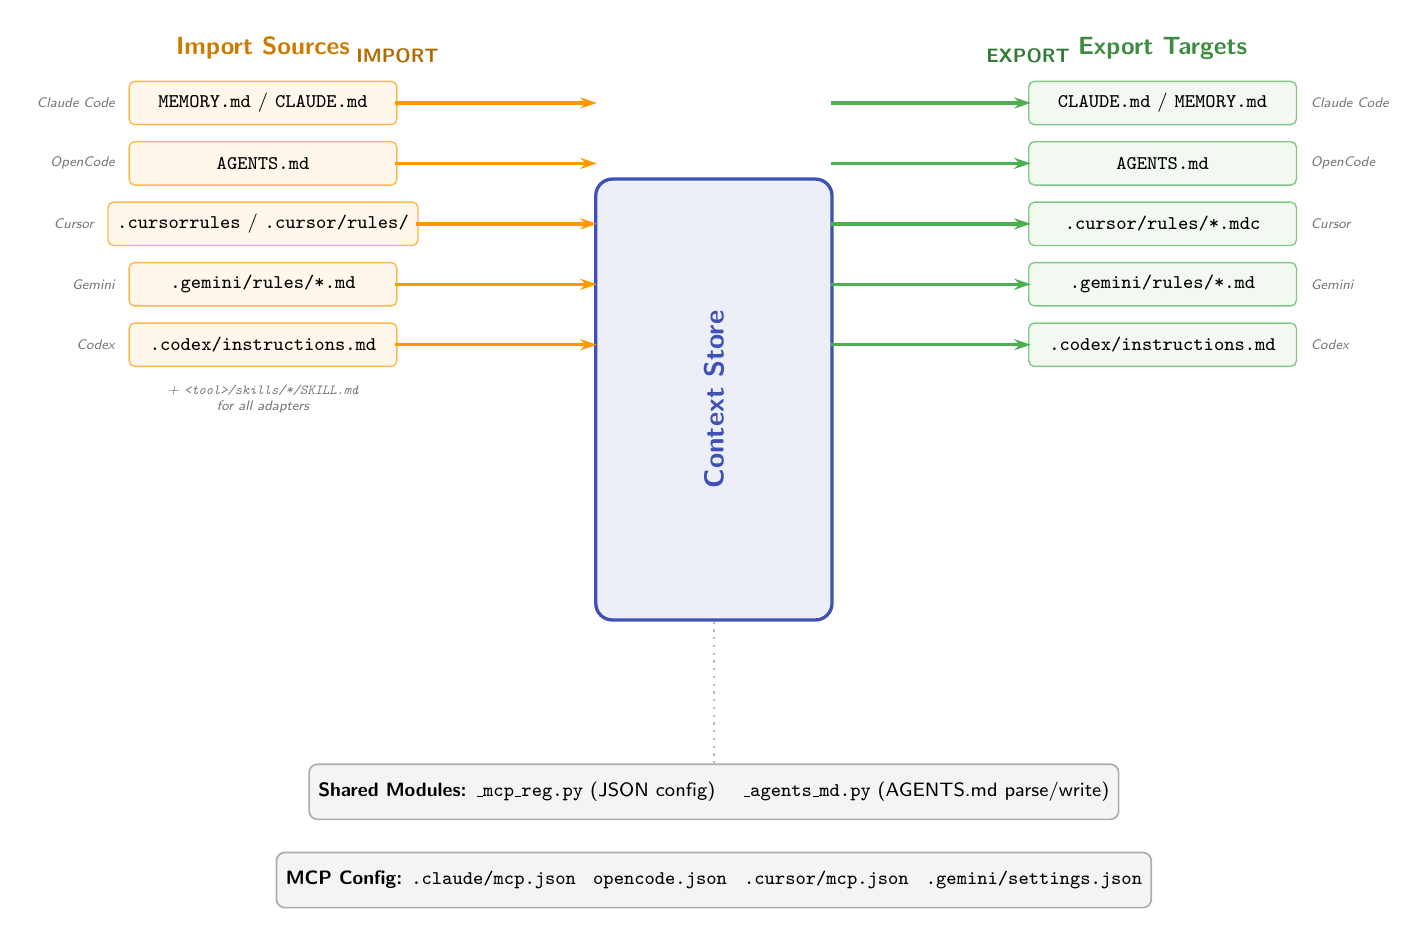
\begin{tikzpicture}[
    >=Stealth,
    every node/.style={font=\sffamily\small},
    filebox/.style={
        draw=adaptorange!70, fill=adaptorange!8, rounded corners=2pt,
        minimum width=3.4cm, minimum height=0.55cm,
        line width=0.5pt, font=\sffamily\scriptsize, align=center
    },
    outbox/.style={
        draw=ifgreen!70, fill=ifgreen!8, rounded corners=2pt,
        minimum width=3.4cm, minimum height=0.55cm,
        line width=0.5pt, font=\sffamily\scriptsize, align=center
    },
    centerbox/.style={
        draw=coreindigo, fill=coreindigo!10, rounded corners=6pt,
        minimum width=3cm, minimum height=5.6cm,
        line width=1.2pt
    },
    modbox/.style={
        draw=fsgray!60, fill=fsgray!8, rounded corners=3pt,
        minimum width=4cm, minimum height=0.7cm,
        line width=0.6pt, font=\sffamily\scriptsize, align=center
    },
    arr/.style={-{Stealth[length=6pt, width=4pt]}, line width=1.2pt, color=#1,
        shorten >=-1pt, shorten <=-1pt},
]

% === Center: Context Store ===
\node[centerbox] (store) {};
\node[font=\sffamily\normalsize\bfseries, text=coreindigo, rotate=90]
    at (store.center) {Context Store};

% === Left: Import sources ===
\node[font=\sffamily\small\bfseries, text=adaptorange!80!black, above left=4.2cm and 4.5cm of store.center]
    (importlabel) {Import Sources};

\node[filebox, below=0.15cm of importlabel] (im1) {\texttt{MEMORY.md} / \texttt{CLAUDE.md}};
\node[filebox, below=0.2cm of im1] (im2) {\texttt{AGENTS.md}};
\node[filebox, below=0.2cm of im2] (im3) {\texttt{.cursorrules} / \texttt{.cursor/rules/}};
\node[filebox, below=0.2cm of im3] (im4) {\texttt{.gemini/rules/*.md}};
\node[filebox, below=0.2cm of im4] (im5) {\texttt{.codex/instructions.md}};

% Tool labels on the left
\node[font=\sffamily\tiny\itshape, text=fsgray, left=0.05cm of im1.west, anchor=east] {Claude Code};
\node[font=\sffamily\tiny\itshape, text=fsgray, left=0.05cm of im2.west, anchor=east] {OpenCode};
\node[font=\sffamily\tiny\itshape, text=fsgray, left=0.05cm of im3.west, anchor=east] {Cursor};
\node[font=\sffamily\tiny\itshape, text=fsgray, left=0.05cm of im4.west, anchor=east] {Gemini};
\node[font=\sffamily\tiny\itshape, text=fsgray, left=0.05cm of im5.west, anchor=east] {Codex};

% Import arrows
\foreach \n in {im1,im2,im3,im4,im5} {
    \draw[arr=adaptorange] (\n.east) -- (store.west |- \n.east);
}

% Import label arrow
\node[font=\sffamily\scriptsize\bfseries, text=adaptorange!70!black,
    above=0.1cm of im1.north east, anchor=south] {IMPORT};

% === Right: Export targets ===
\node[font=\sffamily\small\bfseries, text=ifgreen!80!black, above right=4.2cm and 4.5cm of store.center]
    (exportlabel) {Export Targets};

\node[outbox, below=0.15cm of exportlabel] (ex1) {\texttt{CLAUDE.md} / \texttt{MEMORY.md}};
\node[outbox, below=0.2cm of ex1] (ex2) {\texttt{AGENTS.md}};
\node[outbox, below=0.2cm of ex2] (ex3) {\texttt{.cursor/rules/*.mdc}};
\node[outbox, below=0.2cm of ex3] (ex4) {\texttt{.gemini/rules/*.md}};
\node[outbox, below=0.2cm of ex4] (ex5) {\texttt{.codex/instructions.md}};

% Tool labels on the right
\node[font=\sffamily\tiny\itshape, text=fsgray, right=0.05cm of ex1.east, anchor=west] {Claude Code};
\node[font=\sffamily\tiny\itshape, text=fsgray, right=0.05cm of ex2.east, anchor=west] {OpenCode};
\node[font=\sffamily\tiny\itshape, text=fsgray, right=0.05cm of ex3.east, anchor=west] {Cursor};
\node[font=\sffamily\tiny\itshape, text=fsgray, right=0.05cm of ex4.east, anchor=west] {Gemini};
\node[font=\sffamily\tiny\itshape, text=fsgray, right=0.05cm of ex5.east, anchor=west] {Codex};

% Export arrows
\foreach \n in {ex1,ex2,ex3,ex4,ex5} {
    \draw[arr=ifgreen] (store.east |- \n.west) -- (\n.west);
}

% Export label arrow
\node[font=\sffamily\scriptsize\bfseries, text=ifgreen!70!black,
    above=0.1cm of ex1.north west, anchor=south] {EXPORT};

% === Bottom: Shared Modules ===
\node[modbox, minimum width=8cm, below=1.8cm of store.south] (shared)
    {\textbf{Shared Modules:} \texttt{\_mcp\_reg.py} (JSON conf{}ig) \quad \texttt{\_agents\_md.py} (AGENTS.md parse/write)};

% MCP config paths
\node[modbox, minimum width=8cm, below=0.4cm of shared] (mcpconf)
    {\textbf{MCP Conf{}ig:} \texttt{.claude/mcp.json} \enspace \texttt{opencode.json} \enspace \texttt{.cursor/mcp.json} \enspace \texttt{.gemini/settings.json}};

% Arrows to shared
\draw[dotted, thick, color=fsgray!50] (store.south) -- (shared.north);

% All adapters skills note
\node[font=\sffamily\tiny\itshape, text=fsgray, below=0.1cm of im5.south, align=center]
    {+ \texttt{<tool>/skills/*/SKILL.md}\\for all adapters};

\end{tikzpicture}
\end{document}
